\documentclass[unicode, notheorems]{beamer}
\mode<presentation>
{
	\usetheme[numbers, totalnumbers, minimal]{Statmod}
	\setbeamercovered{transparent}
	\setbeamertemplate{caption}[numbered]
	\setbeamertemplate{enumerate item}[default]
	\setbeamertemplate{itemize item}[circle]
}

\usepackage{tikz}
\usepackage[T2A]{fontenc}
\usepackage[utf8]{inputenc}
\usepackage[russian]{babel}
\usepackage{amsthm}
\usepackage{graphicx}
\usepackage{tikzscale}
\usepackage{float}
\usepackage{subfig}
\usepackage{bm}

\DeclareMathOperator{\E}{\mathbb{E}}
\DeclareMathOperator{\Prb}{\mathbb{P}}
\DeclareMathOperator*{\argmax}{arg\,max\ }

\setbeamertemplate{navigation symbols}{}

\title[Оценивание расстояния на графах де Брёйна]{Задачи оценивания геномного расстояния на графах де Брёйна}

\author[Константинов А. В., гр. 15.Б04-мм]{Константинов Антон Владимирович, гр. 15.Б04-мм}
\institute[СПбГУ]{
	\small
	Санкт-Петербургский государственный университет \\
	Прикладная математика и информатика \\
	Вычислительная стохастика и статистические модели \\
	\vspace{0.4cm}
	Научный руководитель: к.ф.-м.н., доцент Коробейников~А. И. \\
	Рецензент: м.н.с. Шлемов~А. Ю.
	\vspace{0.3cm}
}
\date{
	Санкт-Петербург\\
	2019
}

\begin{document}

\begin{frame}
	\titlepage
\end{frame}

\begin{frame}{Сборка генома}
	\begin{block}{}
  		\textbf{Геном} --- строка над конечным алфавитом $\{ \mathbf{A}, \mathbf{C}, \mathbf{G}, \mathbf{T} \}$.
  	\end{block}
    \begin{itemize}
	   \item  Размеры геномов у различных биологических видов варьируются в диапазоне от 100 тыс.  до  150 млрд. символов.
	   \item Не существует метода, позволяющего прочитать геном целиком.
	   \item Вместо этого из генома случайным образом считываются подстроки, называемые \textit{ридами}. Мы будем иметь дело с \textit{короткими} ридами, имеющими длину 50--200 символов. 
	   \item Исходный геном затем <<собирается>> по перекрытиям ридов.
	\end{itemize}
\end{frame}

\begin{frame}[fragile]{Граф де Брёйна}
	\begin{block}{}
		$k$-мер строки $S$ --- это её подстрока длины $k$.
	\end{block}
	\medskip
    \begin{minipage}{0.6\textwidth}
        \textbf{Граф де Брёйна $G$, $k \in \mathbb{N}$}:
        \begin{enumerate}
            \item Вершины --- $k$-меры строки $\mathcal{S}$.
            \item $u$ и $v$ соединены ребром кратности $N$, если $\mathcal{S}$ содержит $N$ раз встречающийся $(k+1)$-мер, имеющий префикс $u$ и суффикс $v$.
        \end{enumerate}
		
        Хорошо известно, что в $G$ существует \textit{эйлеров} (проходящий по всем рёбрам столько раз, какова их кратность) путь $\mathbf{p}$, который соответствует $\mathcal{S}$.
    \end{minipage}%
    \begin{minipage}{0.4\textwidth}
%   		\scalebox{0.8\textwidth}{$\mathcal{S} = \mathrm{AACTATACTAGACT}$, $k=3$}
    	\begin{figure}
	        \centering
    	    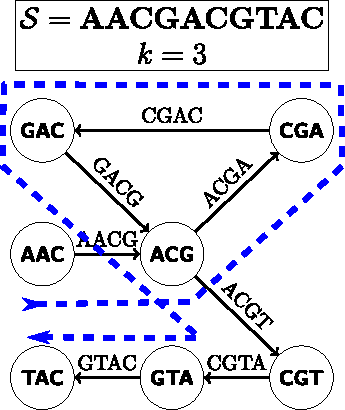
\includegraphics[width=0.9\linewidth]{fig/dBg}
        \end{figure}
    \end{minipage}
	
	\bigskip
    Сборка генома $\iff$ поиск $\mathbf{p}$ среди всех эйлеровых путей в G.
\end{frame}

\begin{frame}{Проблема повторов}
	\textbf{Проблема}: повторы последовательностей (длины $\ge k$) приводят к образованию циклов.
\begin{minipage}{0.6\textwidth}
	
	\bigskip
	Добавим к строке $\mathcal{S}$ из прошлого примера один символ \textbf{\color{red} G} в конец.
	
	\medskip
	Как теперь должен проходить геномный путь: \begin{itemize}
		\item По верхней петле, затем по нижней?
		\item Наоборот, сначала по нижней петле, затем по верхней?
	\end{itemize}
\end{minipage}%
\begin{minipage}{0.4\textwidth}
	\begin{figure}
		\centering
		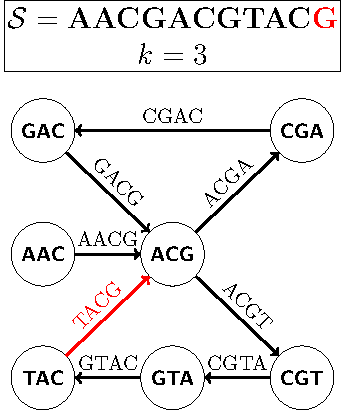
\includegraphics[width=0.9\textwidth]{fig/dBg_repeat}
	\end{figure}
\end{minipage}

\bigskip
По графу ответить на этот вопрос невозможно!

\medskip
Для разрешения повторов обычно используют информацию о расстоянии между рёбрами графа.
\end{frame}

\begin{frame}{Постановка задачи}
	Зафиксируем пару $\mathbf{e}_1, \mathbf{e}_2$ рёбер графа де Брёйна.
	Будем предполагать, что
	\begin{enumerate}
		\item  $\mathbf{e}_1 = \mathcal{S}[a, b]$ и $\mathbf{e}_2 = \mathcal{S}[c, d]$, где $a < c$;
		\item $\mathbf{e}_1$ и $\mathbf{e}_2$ соединяет путь $\bm p =  \mathbf{e}_1 \to p_1 \to \ldots \to p_m \to \mathbf{e}_2$.
	\end{enumerate}
	\bigskip
	{\bf Графовое расстояние:} $d_{\mathrm{graph}} (\mathbf{e}_1, \mathbf{e}_2; \bm p) = \sum_{i=1}^m |p_i| - (m+1)k$,\\
	\medskip
 	{\bf Геномное расстояние:} $d_{\mathrm{genome}}(\mathbf{e}_1, \mathbf{e}_2) = c - b$.\\
 	\bigskip
	Определим множества
	\begin{gather*}
		\mathbf{D}_{\mathrm{graph}} = \big\{ d_{\mathrm{graph}} (\mathbf{e}_1, \mathbf{e}_2; \bm p)\  |\  \bm p \text{ --- путь, соединяющий } \mathbf{e}_1 \text{ с } \mathbf{e}_2  \big\} , \\
		\mathbf{D}_{\mathrm{genome}} = \big\{  d_{\mathrm{genome}}(\mathbf{e}_1^{(i)}, \mathbf{e}_2^{(j)})\ \mid \mathbf{e}_s^{(t)} \text{ --- } t \text{-ое вхождение } \mathbf{e}_s \text{ в геном } \mathcal{S} \big\},
	\end{gather*}\\ 
	\textsc{ \large \color{blue} Задача:}
	Предложить алгоритм, определяющий  элементы множества $\mathbf{D} = \mathbf{D}_{\mathrm{graph}} \cap \mathbf{D}_{\mathrm{genome}}$.
\end{frame}

\begin{frame}{Вероятностная модель парных ридов}

Пусть $\ell > 0$ --- целое число. Рассмотрим независимые случайные величины $\xi \in \{ 1, \ldots, |\mathcal{S}| - \ell\}$ и $\eta > 0$.

\begin{block}{}
	\begin{enumerate}
		\item Фрагмент --- подстрока генома, имеющая вид $\mathcal{S}[\xi, \xi+\eta]$;
		\item Левый рид --- префикс длины $\ell$ фрагмента, т. е. подстрока  $\mathcal{S}[\xi, \xi+\ell]$;
		\item Правый рид --- суффикс длины $\ell$ фрагмента, т.е. подстрока $\mathcal{S}[\xi+\eta-\ell, \xi+\eta]$.
	\end{enumerate}
\end{block}
\begin{figure}[h]
	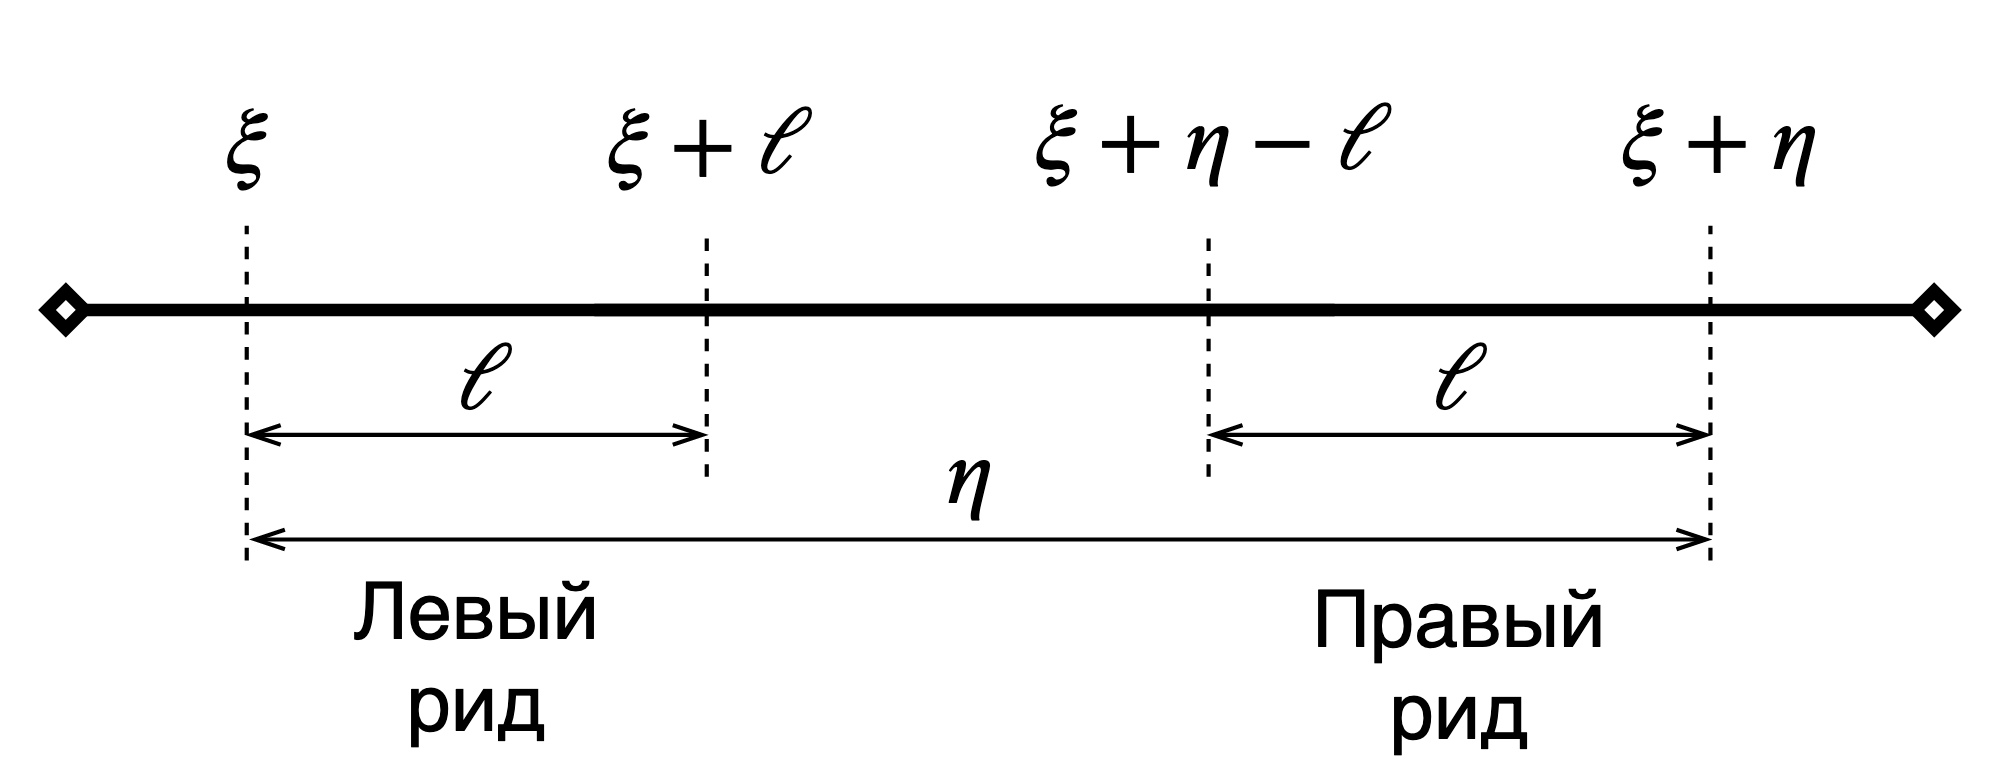
\includegraphics[scale=0.12]{fig/fragment}
	\caption{Структура фрагмента}
\end{figure}
\end{frame}

\begin{frame}{Вероятностный подход к задаче}
	\begin{figure}	
		\centering
		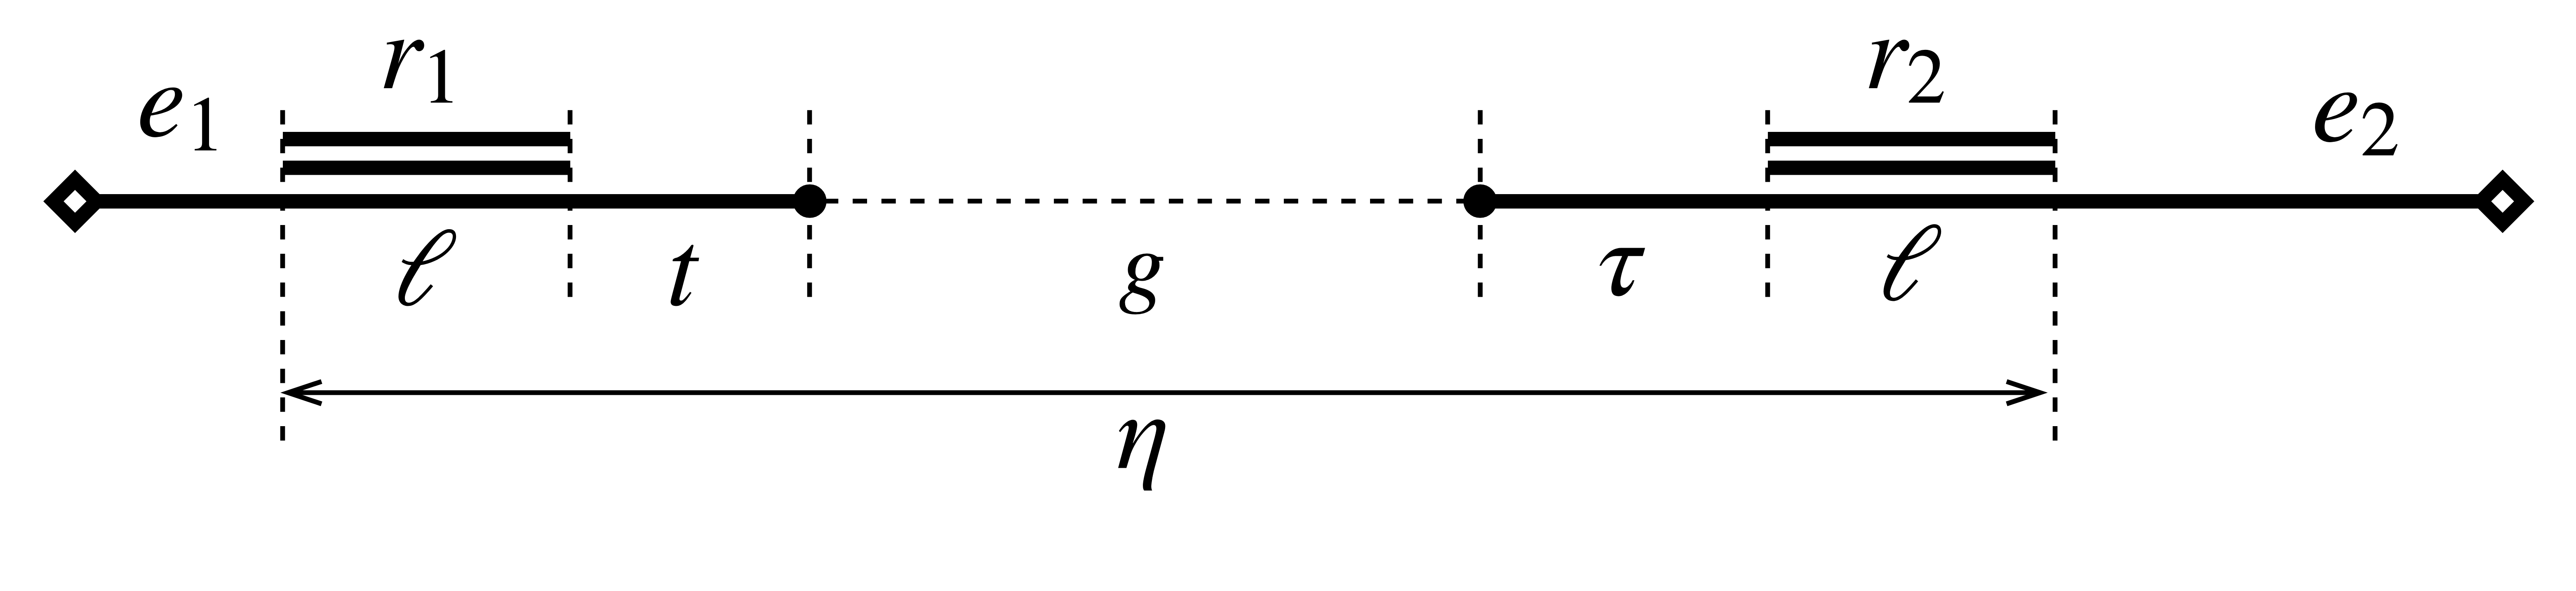
\includegraphics[scale=0.2]{img/alignment_shifted}
		\caption{Расположение ридов на рёбрах графа}
	\end{figure}

	Пусть $(r_1, r_2) \in \mathfrak{R}$, и $r_i$ является подстрокой ребра $\mathbf{e}_i$ ($i=1,2$). \\
	\medskip
	Введём обозначения: 
	\begin{enumerate}
		\item $g$ --- геномное расстояние между $\mathbf{e}_1$ и $\mathbf{e}_2$,
		\item $t$ --- расстояние от конца $r_1$ до конца $\mathbf{e}_1$,
		\item $\tau$ --- координата начала $r_2$ на $\mathbf{e}_2$.
	\end{enumerate}
\end{frame}

\begin{frame}{Вероятностный подход к задаче}
	Рассмотрим формально выборку $\Big( (t_1, \tau_1, g_1), \ldots, (t_n, \tau_n, g_n) \Big)$.
	\begin{enumerate}
		\item Реализации $(t, \tau)$ наблюдаются только при условии $A_{\mathbf{e}_2}(r_2) = \{\text{рид } r_2 \text{ приложен к } \mathbf{e}_2\}$ (будем считать, что $r_1$ уже приложен);
		\item Реализации $g$ не наблюдаются вовсе.
	\end{enumerate}
	\smallskip
	При этом
	\begin{enumerate}
		\item Совместное распределение вектора $(t_i, \tau_i)$ зависит от $g_i$ как от параметра.
		\item $t_i$, $\tau_i$ и $g_i$ связаны соотношением $\tau_i = \eta_i - t_i - g_i - 2\ell$, где $g_i  \in \mathbf{D}$.
	\end{enumerate}
	\smallskip
	Получаем набор реализаций $\mathbb{T} = \Big( (t_1, \tau_1), \ldots, (t_n, \tau_n) \Big)$.\\
	\medskip
	{\color{blue} В этом случае исходная задача сводится к статистическому выводу для $g_i$ по $\mathbb{T}$.}
\end{frame}

\begin{frame}{Апостериорное распределение для одной реализации}
Было получено выражение для функции вероятности $p(g \mid t, \tau, A_{\mathbf{e}_2})$.
\begin{block}{Предложение}
	Пусть длина вставки $\eta$ имеет распределение $\mathcal{P}_\eta$ с функцией распределения $F(x) = \Prb(\eta < x)$. Будем считать, что априорно $g$ равномерно распределена на $\mathbf{D}_{\mathrm{graph}}$.\\
	\medskip
	Тогда
	\begin{equation*}
	\begin{gathered}
	p(g \mid t, \tau,  A_{\mathbf{e}_2}) =  \frac{q(\tau, g, t)}{\sum_{j=1}^k q(\tau, g^{(j)}, t)}	\,,
	\end{gathered}
	\end{equation*}
	где
	\begin{equation*}
		q(x, y, z)  = \frac{F\big(x+y+z+2\ell+1\big) - F\big(x+y+z+2\ell\big)}{F( y + z + \ell + M) - F(y + z + 2\ell)}\,.
	\end{equation*}
\end{block}
\end{frame}

\begin{frame}{Переход к случаю нескольких реализаций}
	\begin{itemize}
		\item На практике для каждого рида  $(r_1, r_2) \in \mathfrak{R}$ реализуется собственное расстояние $g^{(i)} \in \mathbf{D}_{genome}$ для некоторого $i$.
		\item Поэтому нельзя напрямую сделать переход к повторной независимой выборке, как это обычно бывает в статистике.
	\end{itemize}
	\medskip
	Приходим к {\color{blue} модели смеси}:
	\begin{equation*}
		(t, \tau) \sim \sum_{i=1}^k \pi_i  \mathcal{L}_{\tau, t} \big(g^{(i)}\big), \text{ где } \pi_i \ge 0 \text{ и } \sum_{i=1}^k \pi_i = 1.
	\end{equation*}
	Здесь $\pi_i$ мы можем оценить, усредняя апостериорную вероятность $p(g^{(i)} \mid t, \tau, A_{\mathbf{e}_2})$ по всем имеющимся реализациям.
\end{frame}

\begin{frame}{Данные}			
		Во всех тестах использовались графы де Брёйна, построенные по различным библиотекам ридов для первых 400 тысяч нуклеотидов генома \textit{E.coli} (штамм \textit{K12 MG1655}).
		\medskip
		
		Были проведены эксперименты на:\\
		\smallskip
		\textbf{Синтетических ридах} с длиной вставки $\eta \sim \mathrm{N}(\mu, \sigma^2)$:
		\begin{itemize}
			\item $\mu = 1000$, $\sigma = 30$.
			\item $\mu = 400$, $\sigma = 30$.
		\end{itemize}
		\textbf{Реальных ридах}. Были рассмотрены две библиотеки:
		\begin{itemize}
				\item Первая имеет близкое к нормальному распределение $\eta$. Использовалась ф. р. нормального распределения с оценёнными параметрами ($\mu \approx 215$, $\sigma \approx 10$).
				\item Для второй библиотеки в качестве $F$ использовалась эмпирическая ф. р. ($\mathrm{med}\ \eta \approx 480$).
		\end{itemize}
\end{frame}

\begin{frame}{Пример: описание библиотеки}
	Рассмотрим условия, максимально приближенные к реальным:
	\medskip
	
	\begin{minipage}{0.55\textwidth}
		\begin{itemize}
			\item Медианная длина вставки: 480.
			\item В качестве функции распределения $F$, требуемой для получения оценок, мы будем использовать эмпирическую ф. р., полученную по всем имеющимся ридам.
		\end{itemize}
	\end{minipage}%
	\begin{minipage}{0.45\textwidth}
	\begin{figure}
		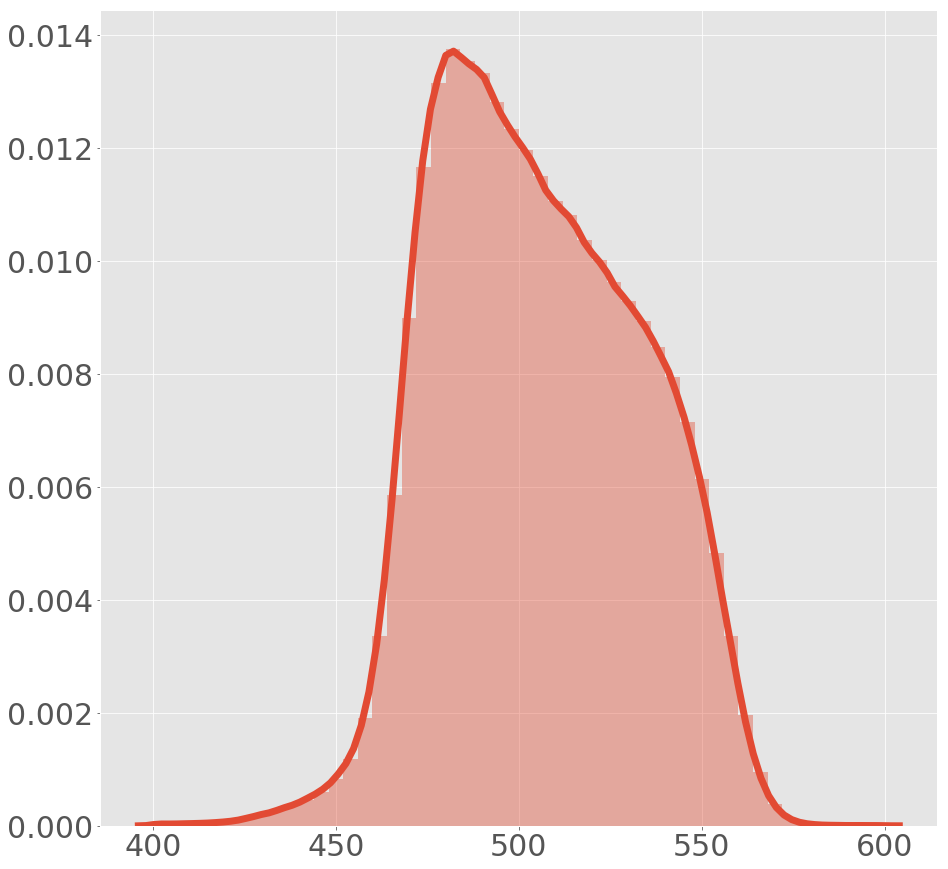
\includegraphics[width=0.9\textwidth]{fig/real-reads/bad-lib/hist}
		\caption{Распределение длины вставки $\eta$}
	\end{figure}
	\end{minipage}
\end{frame}

\begin{frame}{Пример: рёбра без повторов}
\begin{figure}%
	\centering
	\subfloat[Фрагмент графа]{{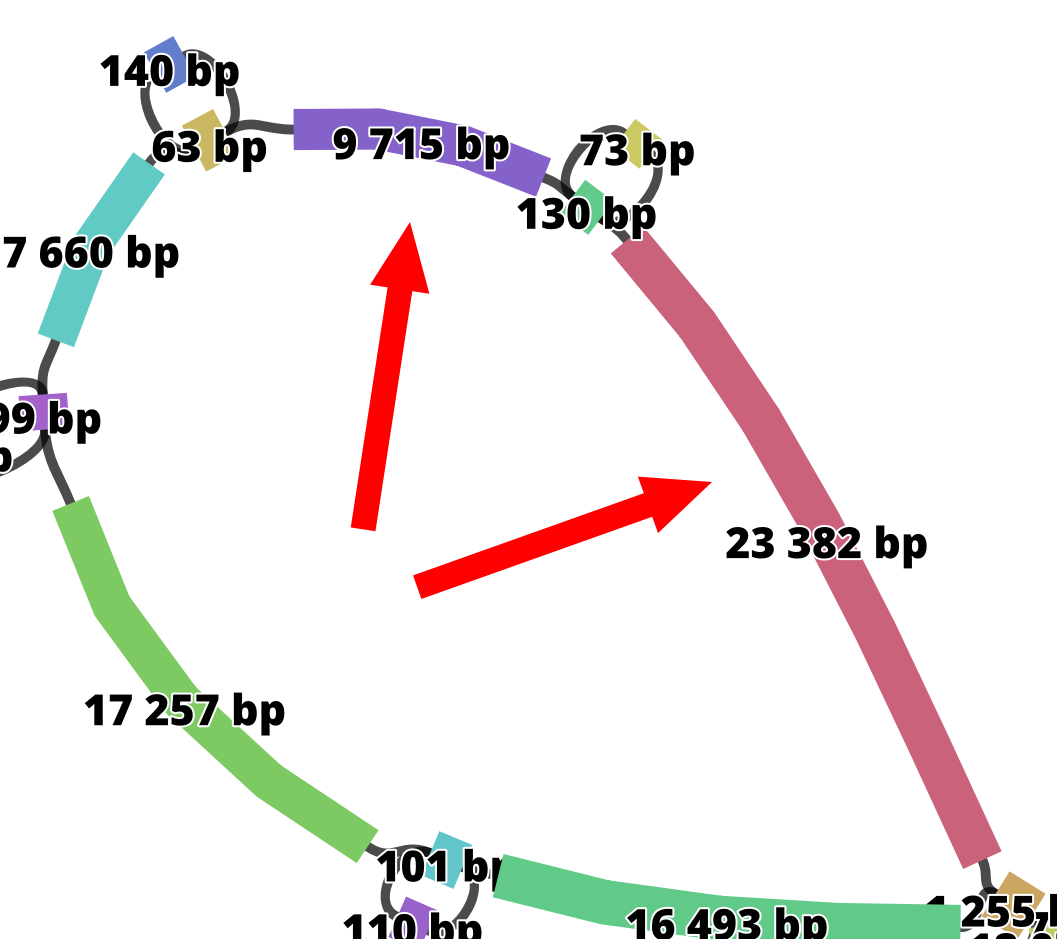
\includegraphics[width=0.45\textwidth]{fig/real-reads/bad-lib/4-graph} }}%
	\qquad
	\subfloat[Апостериорное распределение]{{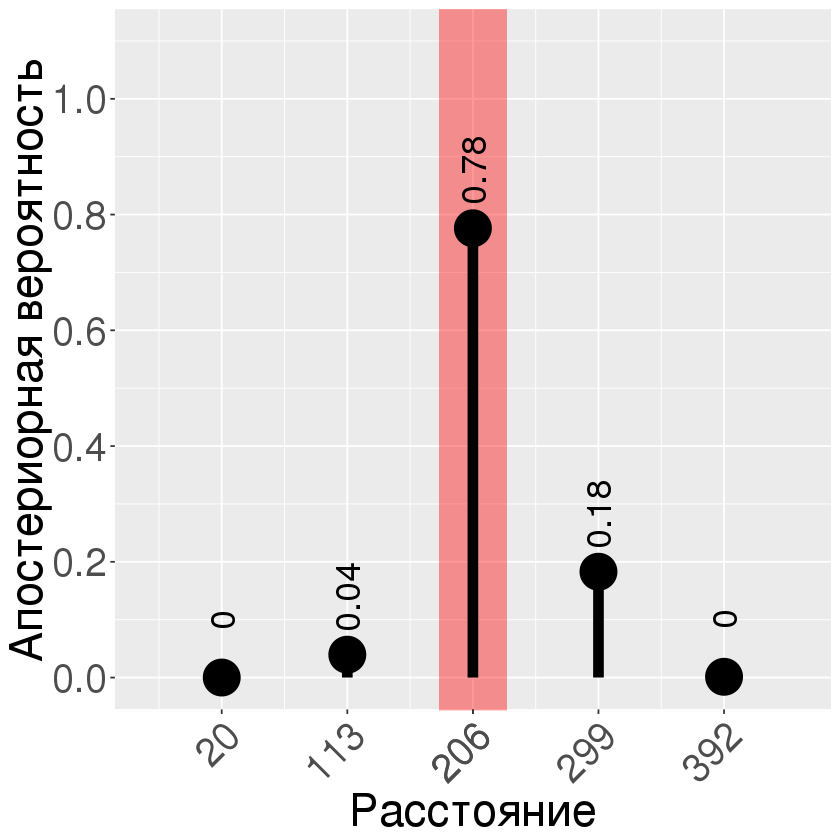
\includegraphics[width=0.45\linewidth]{fig/real-reads/bad-lib/4-posterior} }}%
	\caption{Два длинных ребра, не имеющих повторов}
\end{figure}
\end{frame}

\begin{frame}{Пример: повторное ребро}
\begin{figure}%
	\centering
	\subfloat[Фрагмент графа]{{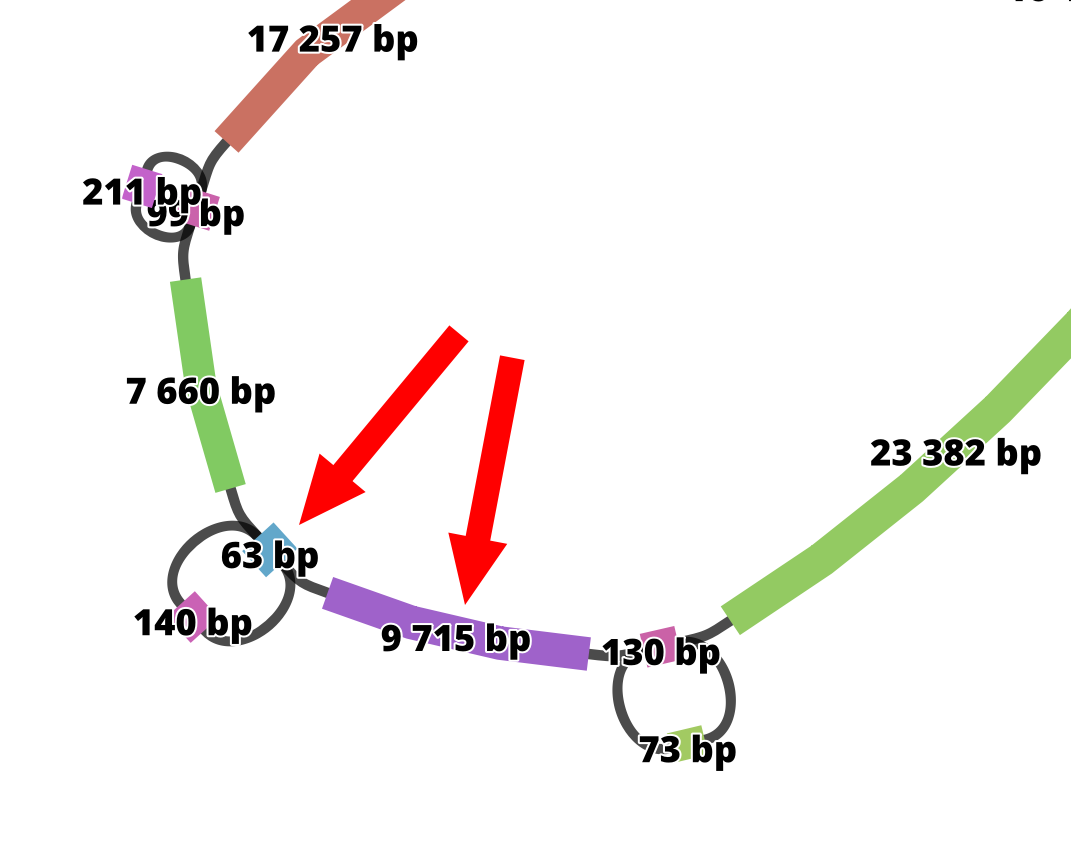
\includegraphics[width=0.45\linewidth]{fig/real-reads/bad-lib/3-graph} }}%
	\qquad
	\subfloat[Гистограмма $\eta - g$]{{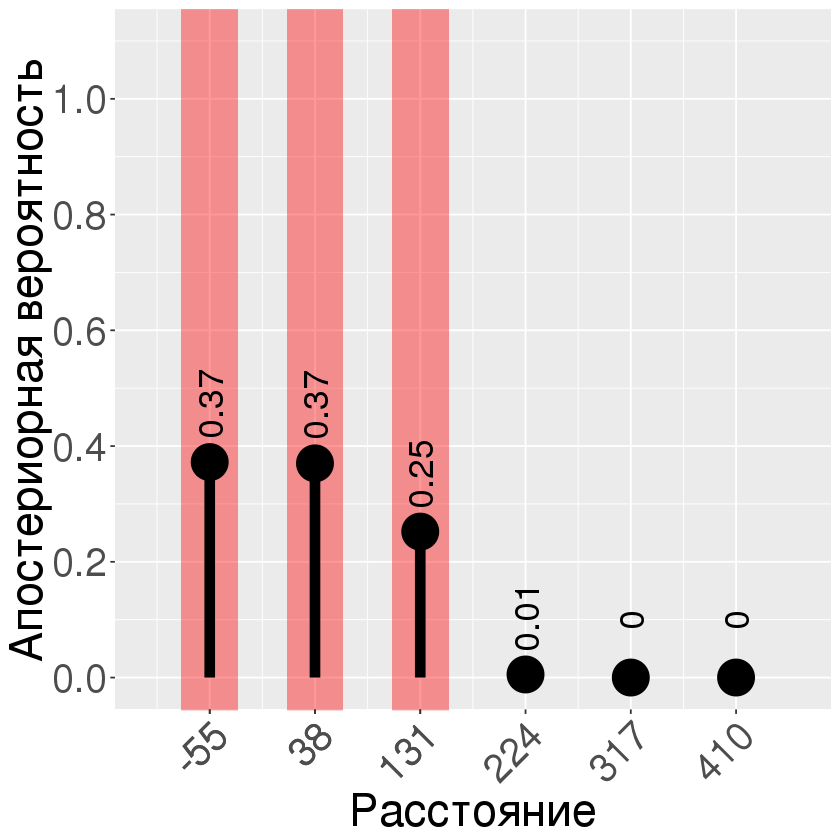
\includegraphics[width=0.45\linewidth]{fig/real-reads/bad-lib/3-posterior} }}%
	\caption{Длинное ребро без повторов и короткое ребро (63 bp) тройной кратности}
\end{figure}
\end{frame}

\begin{frame}{Заключение}
	В работе была рассмотрена задача оценки геномных расстояний между рёбрами в графе де Брёйна.
	\bigskip
	\begin{enumerate}
		\item Построена вероятностная модель, позволяющая получать требуемые оценки в виде апостериорных вероятностей для расстояний, имеющихся в графе.
		\item Построенная модель протестирована на реальных геномных данных.
	\end{enumerate}
	\bigskip
	В дальнейшем полученные оценки, например, могут быть применены в геномных ассемблерах для разрешения повторов в графе де Брёйна. 
\end{frame}

\end{document}
